\documentclass[aspectratio=169,10pt]{beamer}
\usepackage{mathptmx}
\usepackage{booktabs}
\usepackage{graphicx}
\usepackage{tikz}
% strike-through (ulem is not installed): a line across the middle of the text
\newcommand{\strike}[1]{\tikz[baseline=(s.base)]{\node[inner sep=0pt,outer sep=0pt](s){#1};\draw[line width=1.2pt]([yshift=0.15ex]s.west)--([yshift=0.15ex]s.east);}}
\usetikzlibrary{calc}
\usefonttheme{serif}
\setbeamertemplate{navigation symbols}{}
\setbeamertemplate{footline}{\hfill\tiny\insertframenumber\hspace{6pt}\vspace{4pt}}
\setbeamercolor{frametitle}{fg=black}
\definecolor{tumblue}{HTML}{0065BD}
\setbeamerfont{frametitle}{size=\normalsize,series=\bfseries}
\setbeamertemplate{itemize items}{\textbullet}
\graphicspath{{../../figures/}{./}}

\begin{document}
% Title slide for text/slides/motivation_slides.tex
\begin{frame}[plain]
\centering
\vspace*{-4pt}
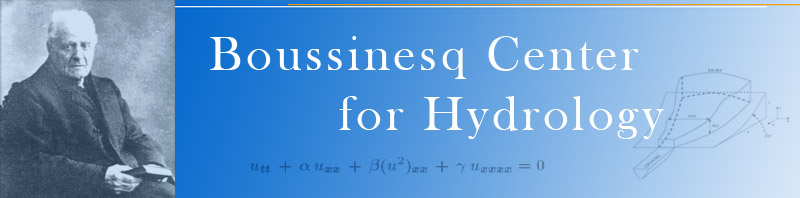
\includegraphics[width=0.62\linewidth]{BC_logo.jpg}\par
\vspace{16pt}
{\Large\bfseries Daily soil moisture at three depths from multimodal drivers\\[3pt] and geospatial foundation model embeddings}\par
\vspace{14pt}
{\large\bfseries Prajwal Khanal}\par
\vspace{12pt}
{\small
\begin{tabular}{@{}l@{\hspace{10pt}}l@{}}
\multicolumn{2}{@{}c@{}}{\textbf{Supervisors}}\\[2pt]
prof.dr. Z.\ Su (Bob)       & Faculty ITC, University of Twente \\
dr. Y.\ Zeng (Yijian)       & Faculty ITC, University of Twente \\
Joost Beckers               & Planet Labs \\
\end{tabular}}\par
\vspace{14pt}
{\small 8 October 2026}
\end{frame}

% Motivation slides 1-4, shared by text/research_questions_slides.tex and text/slides/motivation_slides.tex
\begin{frame}{Motivation\quad Different ways of obtaining soil moisture}
\scriptsize
\centering
\renewcommand{\arraystretch}{1.25}
\begin{tabular}{@{}p{0.14\textwidth} p{0.26\textwidth} p{0.16\textwidth} p{0.34\textwidth}@{}}
\toprule
Source & How SM is obtained & Depth & Main limitation \\
\midrule
\textbf{Microwave}\newline (SMAP, SMOS, ASCAT, S1)
  & invert:\newline $\sigma^0$ or $T_B = f(\mathrm{SM}, \text{roughness}, \text{vegetation})$
  & top $\sim$5\,cm; informs part of the root zone (Feldman et al., 2023)
  & shallow; assumes vegetation and roughness; coarse (9--40\,km) except S1 \\
\addlinespace[7pt]
\textbf{Optical / thermal}\newline (S2, Landsat, MODIS)
  & empirical relations with surface properties: reflectance and indices; LST--vegetation space (e.g. triangle method, TVDI)
  & skin / surface
  & indirect, site-specific calibration; clouds; canopy hides the soil \\
\addlinespace[7pt]
\textbf{Land-surface models}
  & $d\theta/dt = P - ET - Q - D$, with parameters $p$
  & full profile
  & forcing errors, soil and vegetation parameters, process representation (Koster et al., 2009; Seneviratne et al., 2010) \\
\addlinespace[7pt]
\textbf{Reanalysis}\newline (ERA5-Land)
  & LSM driven by reanalysis meteorology
  & full profile
  & model assumptions dominate deep layers with few observational constraints (Li et al., 2021; Miguez-Macho and Fan, 2021) \\
\addlinespace[7pt]
\textbf{In situ} (ISMN)
  & direct probe measurement
  & several depths
  & point scale; sparse, uneven global coverage \\
\addlinespace[7pt]
\textbf{Data-driven}\newline (ML / DL)
  & $\mathrm{SM} = f_\theta(\text{inputs})$, learned from in-situ labels; no ad-hoc process assumptions
  & any depth with labels
  & needs enough, representative sites; generalisation?; hard to interpret? \\
\bottomrule
\end{tabular}
\end{frame}

\begin{frame}{Motivation\quad Multimodal remote sensing}
\begin{columns}[T,onlytextwidth]
\begin{column}{0.56\textwidth}
\centering
\textbf{\footnotesize 1.\ Optical: reflectance spectrum}\\[2pt]
\includegraphics[width=\linewidth,height=0.42\textheight,keepaspectratio]{textbook/sm_signals.pdf}
\scriptsize
\begin{itemize}
\item Dry and wet soil reflect differently: wetting darkens soil in every band, most in the SWIR (B11, B12)
\item Green and water-stressed vegetation reflect differently: stress lowers NIR and raises SWIR
\end{itemize}
\end{column}
\begin{column}{0.41\textwidth}
\centering
\textbf{\footnotesize 2.\ SAR: scattering mechanisms}\\[2pt]
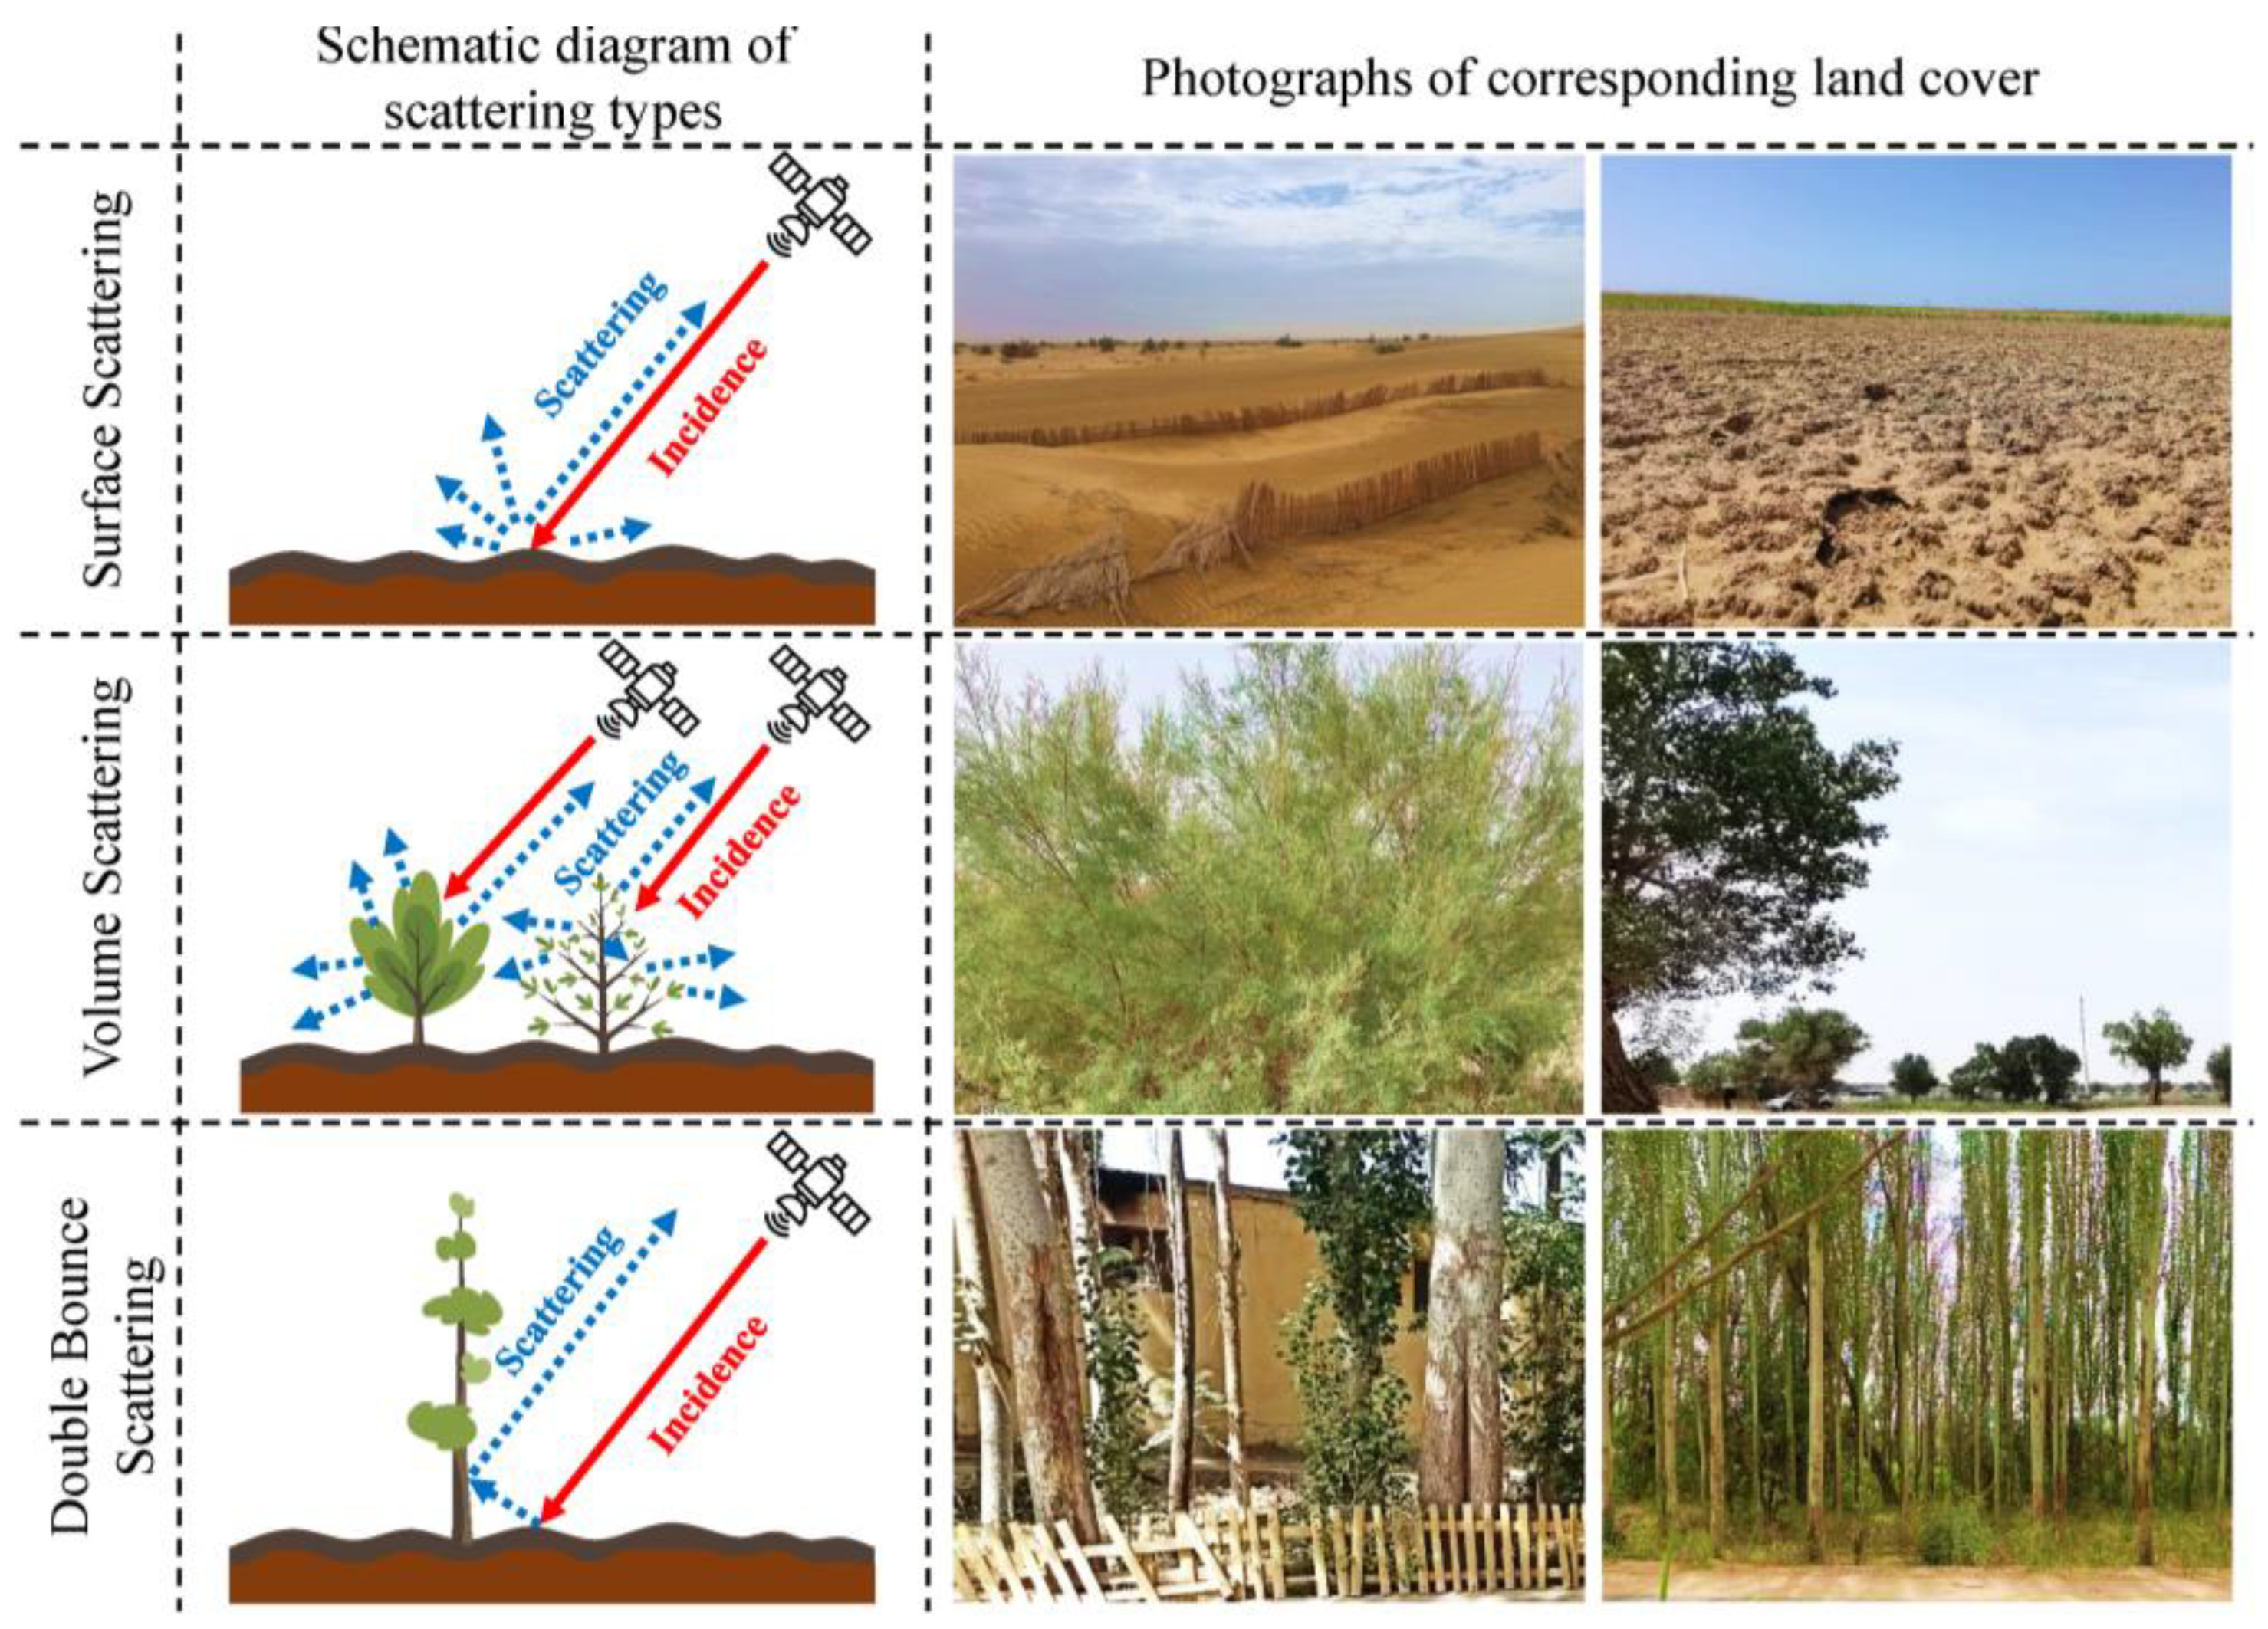
\includegraphics[width=\linewidth,height=0.46\textheight,keepaspectratio]{sensors-25-02512-g003.png}\\[-1pt]
{\tiny Nurmemet et al.\ (2025), \textit{Sensors} 25(8), 2512, doi:10.3390/s25082512}
\scriptsize
\begin{itemize}
\item Bare soil: surface scattering, set by moisture (dielectric) and roughness
\item Canopy: volume and double-bounce scattering mask the soil signal
\end{itemize}
\end{column}
\end{columns}
\end{frame}

\begin{frame}{Motivation\quad Geospatial foundation models (GFMs)}
\centering
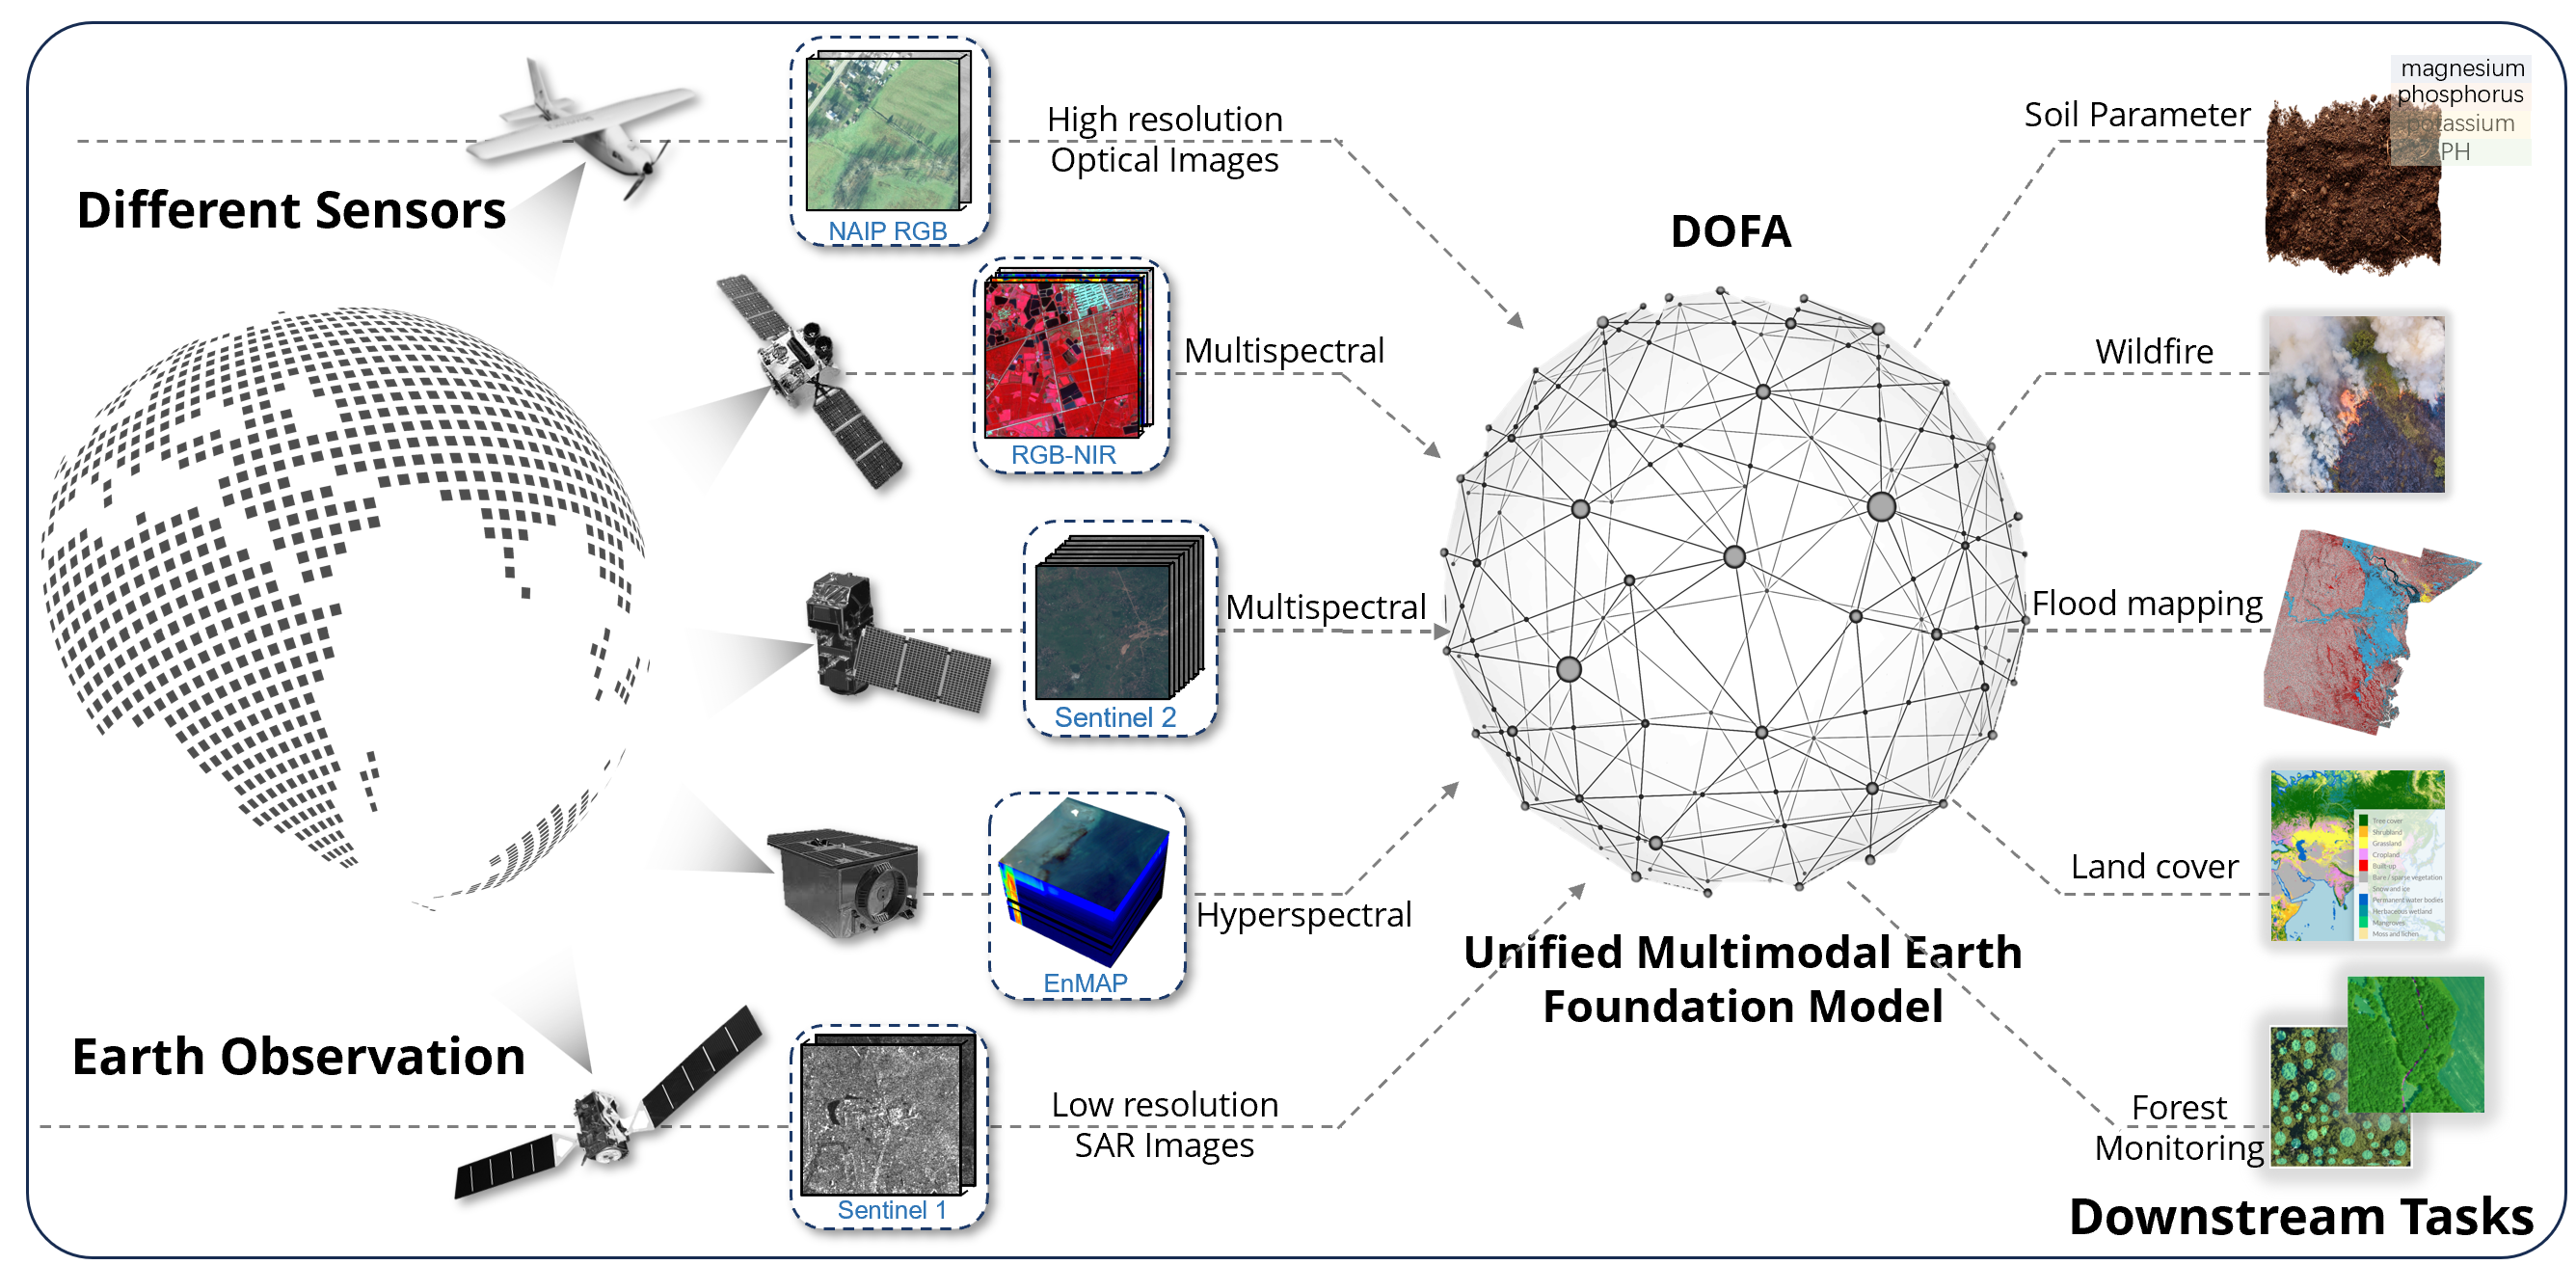
\includegraphics[width=\linewidth,height=0.70\textheight,keepaspectratio]{DOFA1-1.png}\\[-1pt]
{\tiny DOFA: Xiong et al.\ (2024), Neural plasticity-inspired multimodal foundation model for Earth observation, arXiv:2403.15356}\\[6pt]
\begin{beamercolorbox}[wd=0.9\linewidth,center,rounded=true]{block body}
\small\textbf{Once pre-trained on multimodal, unlabelled data, its representation works for many downstream tasks}
\end{beamercolorbox}
\end{frame}

\begin{frame}{Motivation\quad TerraMind embeddings for soil moisture}
\centering
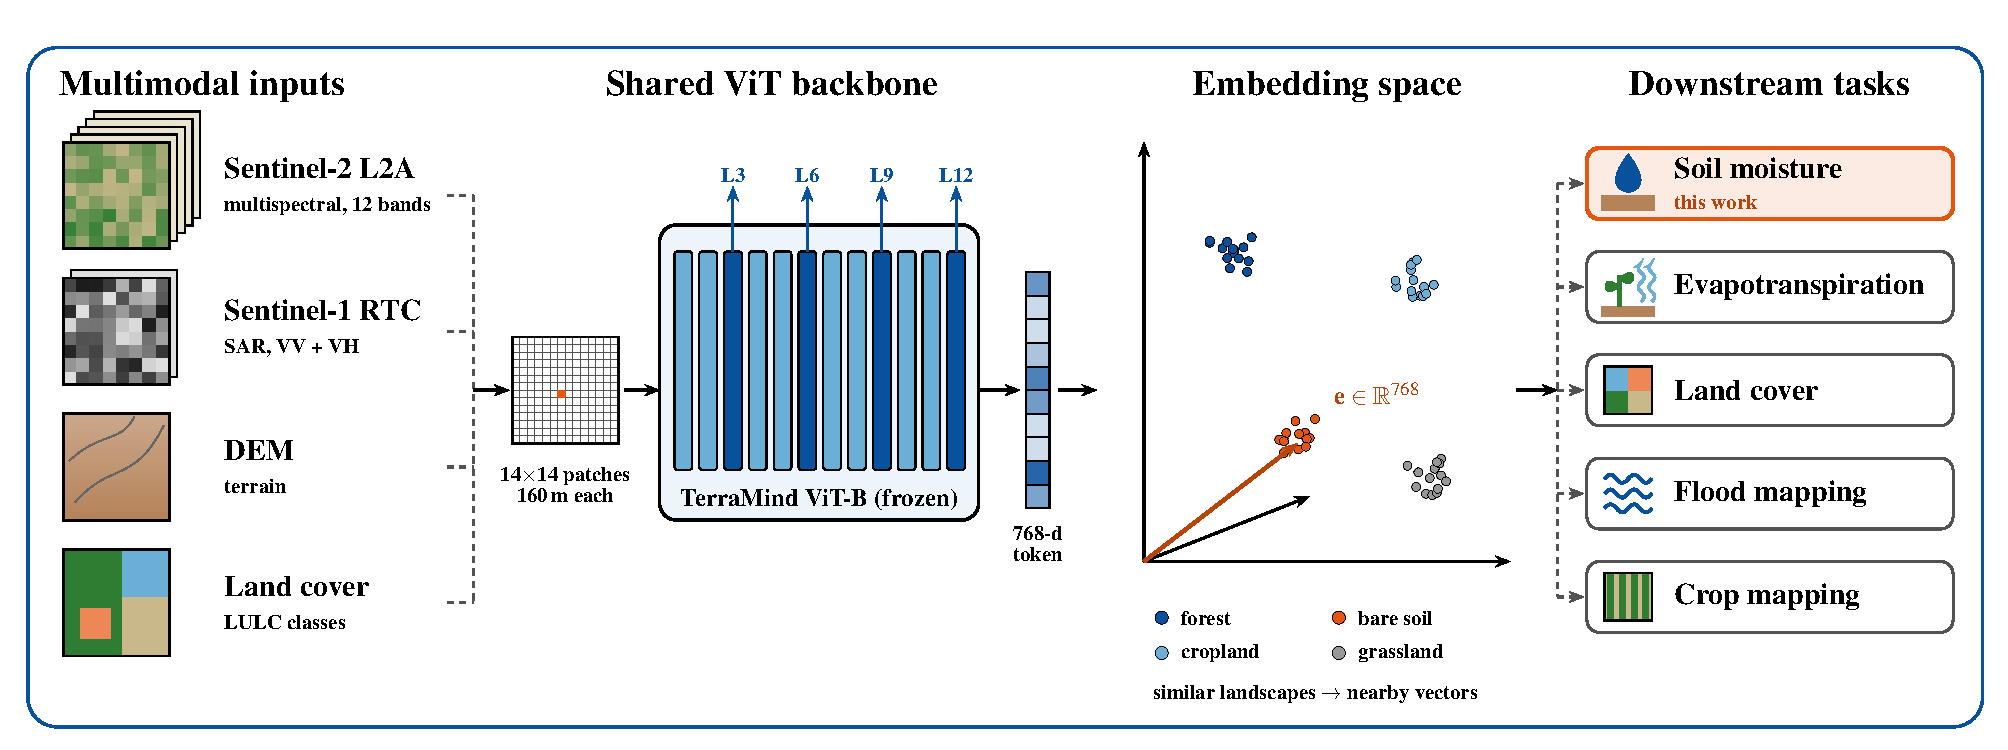
\includegraphics[width=\linewidth,height=0.80\textheight,keepaspectratio]{gfm_embedding_schematic.pdf}\\[4pt]
\footnotesize Frozen TerraMind ViT-B turns each 160\,m patch of S2, S1, DEM and LULC into a 768-d embedding;
the same embedding can serve many tasks; in this case, \textbf{soil moisture}.
\end{frame}

% Architecture slides (method), shared by text/research_questions_slides.tex and text/slides/motivation_slides.tex
% Source figure: figures/architecture_s48/architecture_s48.pdf, 1281.6 x 950.4 bp.
% Overview: the whole figure with the three zoom regions boxed (no words).
% Zoom slides: a large trim-crop of the figure + a thumbnail of the whole figure with everything outside the
% zoomed region shaded and a coloured box on it. Regions are fractions of width / height from the bottom-left.
\definecolor{boxA}{HTML}{E37222}   % inputs  (TUM orange)
\definecolor{boxB}{HTML}{0065BD}   % coarse  (TUM blue)
\definecolor{boxC}{HTML}{A2AD00}   % fine    (TUM green)
% fine-path region in full-figure fractions: from the transformer down, plus the whole bottom band
\def\fineregion{(0,0) -- (1,0) -- (1,0.720) -- (0.575,0.720) -- (0.575,0.245) -- (0,0.245) -- cycle}

% \archthumb{colour}{region}: 2.2 cm thumbnail, drawn at the current point (use inside a tikz node or overlay)
\providecommand{\archthumb}[2]{\begin{tikzpicture}[x={(2.2cm,0)}, y={(0,1.6315cm)}]  % 2.2 cm * 950.4/1281.6
  \node[inner sep=0pt, anchor=south west] at (0,0) {\includegraphics[width=2.2cm]{architecture_s48/architecture_s48.pdf}};
  \fill[black, opacity=0.45, even odd rule] (0,0) rectangle (1,1) #2;
  \draw[black!60, line width=0.3pt] (0,0) rectangle (1,1);
  \draw[#1, line width=1.2pt] #2;
\end{tikzpicture}}
% thumbnail pinned to the top-right corner of the slide
\providecommand{\cornerthumb}[2]{\begin{tikzpicture}[remember picture, overlay]
  \node[anchor=north east, inner sep=0pt] at ([xshift=-0.12cm, yshift=-0.08cm]current page.north east) {\archthumb{#1}{#2}};
\end{tikzpicture}}

\begin{frame}{Method\quad{\color{tumblue}Model architecture}}
\centering
\begin{tikzpicture}[x={(1.34848*0.91\textheight,0)}, y={(0,0.91\textheight)}]
  \node[inner sep=0pt, anchor=south west] at (0,0) {\includegraphics[height=0.91\textheight]{architecture_s48/architecture_s48.pdf}};
  \draw[boxA, line width=1.6pt, rounded corners=3pt] (0.047,0.779) rectangle (0.824,0.962);
  \draw[boxB, line width=1.6pt, rounded corners=3pt] (0.004,0.255) rectangle (0.711,0.754);
  \draw[boxC, line width=1.6pt, rounded corners=3pt] (0.004,0.004) -- (0.996,0.004) -- (0.996,0.716)
        -- (0.579,0.716) -- (0.579,0.241) -- (0.004,0.241) -- cycle;
\end{tikzpicture}
\end{frame}

\begin{frame}{Method\quad{\color{tumblue}Inputs: what the model sees for day D}}
\centering
\includegraphics[width=0.96\linewidth,height=0.86\textheight,keepaspectratio,trim=60 740 225 36,clip]{architecture_s48/architecture_s48.pdf}
\cornerthumb{boxA}{(0.047,0.779) rectangle (0.824,0.962)}
\end{frame}

\begin{frame}{Method\quad{\color{tumblue}Coarse path: tokens $\rightarrow$ transformer}}
\centering
\includegraphics[width=0.96\linewidth,height=0.86\textheight,keepaspectratio,trim=0 235 370 234,clip]{architecture_s48/architecture_s48.pdf}
\cornerthumb{boxB}{(0,0.247) rectangle (0.711,0.754)}
\end{frame}

% Fine path: full-page crop of the bottom 72 % (trim top 266 bp); everything up to the transformer is shaded and
% the thumbnail sits inside that shaded area. Box / fade coordinates are fractions of the CROP.
\begin{frame}{Method\quad{\color{tumblue}Fine path: 20\,m CNN $\rightarrow$ U-Net decoder $\rightarrow$ depth heads}}
\centering
\begin{tikzpicture}[x={(1.87287*0.84\textheight,0)}, y={(0,0.84\textheight)}]  % crop is 1281.6 x 684.4 bp
  \node[inner sep=0pt, anchor=south west] at (0,0) {\includegraphics[height=0.84\textheight,trim=0 0 0 266,clip]{architecture_s48/architecture_s48.pdf}};
  \fill[white, opacity=0.78] (0,0.340) -- (0.575,0.340) -- (0.575,1) -- (0,1) -- cycle;
  \node[anchor=north west, inner sep=0pt] at (0.02,0.98) {\archthumb{boxC}{\fineregion}};
  \begin{scope}[boxC, line width=1.4pt, rounded corners=3pt]
    \draw (0.003,0.054) rectangle (0.235,0.304);   % fine inputs + stems
    \draw (0.240,0.063) rectangle (0.495,0.299);   % GroupNorm CNN encoder
    \draw (0.578,0.515) rectangle (0.672,0.996);   % transformer (bottleneck + context)
    \draw (0.600,0.100) rectangle (0.862,0.327);   % U-Net decoder
    \draw (0.868,0.136) rectangle (0.997,0.905);   % depth heads, maps, Huber loss
  \end{scope}
\end{tikzpicture}
\end{frame}

% Data slides, shared by text/research_questions_slides.tex and text/slides/prajwal_khanal_uTwente_ITC.tex.
% Style as motivation slides 2-5: figure -> one-line caption (\figcap) -> one-line message in a rounded box (\msg).
% Figures: figures/eval/baseline_selected_20261005_paper/ (data_overview 1116 x 864 bp; stations_by_* 685.2 x 267.6 bp).
% Numbers: data_overview_points.csv (observed station-days), satellite_zarr/*/{s2,s1_asc,s1_desc}/dates/.zarray shapes (scene counts),
% text/logs.txt splice dry run (ERA5 station-days).

\begin{frame}{Data\quad{\color{tumblue}In-situ soil moisture: global coverage}}
\centering
\includegraphics[width=\linewidth,height=0.66\textheight,keepaspectratio,trim=0 434 0 0,clip]{eval/baseline_selected_20261005_paper/data_overview.pdf}
\figcap{886 soil-moisture stations (ISMN and flux sites): train 573, validation 89, out-of-sample (OOS) 224}
\msg{Dense in North America and Europe; sparse in the tropics and the Southern Hemisphere}
\end{frame}

\begin{frame}{Data\quad{\color{tumblue}Depth coverage, record length and splits}}
\centering
\includegraphics[width=\linewidth,height=0.64\textheight,keepaspectratio,trim=0 0 0 455,clip]{eval/baseline_selected_20261005_paper/data_overview.pdf}
\figcap{(b) train / validation / OOS stations, time cut 2023-01-01; (c) observed record per station; (d) observed station-days}
\msg{0--10 cm: 885 stations (median 6.2 yr); 10--30 cm: 682 (6.6 yr); 30--100 cm: 551 (6.6 yr)}
\end{frame}

\begin{frame}{Data\quad{\color{tumblue}Climate and land-cover coverage}}
\centering
\includegraphics[width=0.49\linewidth,trim=0 0 340 0,clip]{eval/baseline_selected_20261005_paper/stations_by_kg_macro.pdf}\hfill
\includegraphics[width=0.49\linewidth,trim=0 0 340 0,clip]{eval/baseline_selected_20261005_paper/stations_by_igbp_macro.pdf}
\figcap{Stations per K\"oppen climate zone (left) and land-cover class (right), by split}
\msg{Mostly continental, temperate and arid; forest and grass-crop; almost no tropics or polar}
\end{frame}

\begin{frame}{Data\quad{\color{tumblue}Data points in total}}
\centering\small
\renewcommand{\arraystretch}{1.3}
\begin{tabular}{@{}l l@{}}
\toprule
\textbf{Stations} & 990 in inventory; \textbf{886} with soil moisture (train 573 / val 89 / OOS 224) \\
\textbf{Depths} & 0--10 cm: 885 \quad 10--30 cm: 682 \quad 30--100 cm: 551 stations \\
\textbf{Period} & 2016--2025; out-of-time test from 2023-01-01 \\
\textbf{Soil-moisture observations} & \textbf{5.14\,M} observed daily values (2.10\,M / 1.68\,M / 1.37\,M per depth) \\
\textbf{Sentinel-2 L2A} & 272,281 scenes (994 sites); cloud $<$ 75\,\% per scene, cloudy tokens masked \\
\textbf{Sentinel-1 RTC} & 496,835 scenes: 251,310 ascending + 245,525 descending \\
\textbf{ERA5-Land} & 18 variables, 2.46\,M station-days (990 stations) \\
\textbf{Static / other} & DEM, LULC, soil (OpenLandMap), SIF, TWSA \\
\bottomrule
\end{tabular}
\msg{About 5.1 million daily soil-moisture observations at 886 stations, 0--100 cm}
\end{frame}

% Results slides, shared by text/research_questions_slides.tex and text/slides/motivation_slides.tex.
% Style: figure -> one-line caption (\figcap) -> one-line message in a rounded box (\msg).
% Model: baseline_selected_20261005 (the selected §59 run); figures from figures/eval/baseline_selected_20261005_paper/,
% numbers from eval_output/baseline_selected_20261005/per_station_oos.csv.
% Order (user, 2026-10-07): ubRMSE by depth -> pred vs obs (density) -> ubRMSE by land cover ->
% 3-depth sites that match -> 3-depth sites that do not -> TxSON (tile left, series right).
% Match / mismatch = lowest / highest mean OOS ubRMSE among stations observed at all three depths.

\begin{frame}{Results\quad{\color{tumblue}Per-station ubRMSE by depth}}
\centering
\includegraphics[width=\linewidth,height=0.66\textheight,keepaspectratio]{eval/baseline_selected_20261005_paper/box_ubrmse_by_depth.pdf}
\figcap{One point per station; medians above, station counts below}
\msg{Median per-station ubRMSE 0.043--0.051\,m$^3$/m$^3$ at every depth and split}
\end{frame}

\begin{frame}{Results\quad{\color{tumblue}Predicted vs observed, by split and depth}}
\centering
\includegraphics[width=\linewidth,height=0.68\textheight,keepaspectratio]{eval/baseline_selected_20261005_paper/scatter_pred_obs_kde.pdf}
\figcap{All daily samples, smoothed density; shaded bands hold 50/75/90/99\,\% of samples; rows OOS, OOT, OOST}
\msg{New years at known sites (OOT, r$^2$ 0.70--0.74) fit far better than new sites (r$^2$ 0.29--0.46)}
\end{frame}

\begin{frame}{Results\quad{\color{tumblue}Per-station ubRMSE by land cover}}
\centering
\includegraphics[width=\linewidth,height=0.68\textheight,keepaspectratio]{eval/baseline_selected_20261005_paper/box_ubrmse_by_igbp_macro.pdf}
\figcap{Rows: depths; groups: land-cover class; colours: OOS, OOT, OOST}
\msg{Similar error across land cover; forest slightly highest, shrub--savanna lowest}
\end{frame}

\begin{frame}{Results\quad{\color{tumblue}Sites where all three depths match}}
\centering
\begin{minipage}[t]{0.495\linewidth}\centering
\includegraphics[width=\linewidth,height=0.64\textheight,keepaspectratio]{eval/baseline_selected_20261005_paper/timeseries/oos/BEST_01_ISMN_NGARI_ALI02.png}\\[-1pt]
{\scriptsize\bfseries NGARI ALI02, Tibetan Plateau (best)}
\end{minipage}\hfill
\begin{minipage}[t]{0.495\linewidth}\centering
\includegraphics[width=\linewidth,height=0.64\textheight,keepaspectratio]{eval/baseline_selected_20261005_paper/timeseries/oos/BEST_05_ISMN_SCAN_DoeRidge.png}\\[-1pt]
{\scriptsize\bfseries SCAN Doe Ridge, California}
\end{minipage}
\figcap{OOS stations observed at all three depths, lowest ubRMSE; blue predicted, black observed}
\msg{Dynamics right at all depths (ubRMSE 0.013--0.036, r 0.57--0.73); level off by up to 0.05}
\end{frame}

\begin{frame}{Results\quad{\color{tumblue}Sites where the depths do not match}}
\centering
\begin{minipage}[t]{0.495\linewidth}\centering
\includegraphics[width=\linewidth,height=0.64\textheight,keepaspectratio]{eval/baseline_selected_20261005_paper/timeseries/oos/WORST_02_ISMN_SNOTEL_BurtsMillerRanch.png}\\[-1pt]
{\scriptsize\bfseries SNOTEL Burts Miller Ranch, Utah}
\end{minipage}\hfill
\begin{minipage}[t]{0.495\linewidth}\centering
\includegraphics[width=\linewidth,height=0.64\textheight,keepaspectratio]{eval/baseline_selected_20261005_paper/timeseries/oos/WORST_04_ISMN_SNOTEL_Hopewell.png}\\[-1pt]
{\scriptsize\bfseries SNOTEL Hopewell, New Mexico}
\end{minipage}
\figcap{OOS stations observed at all three depths, highest ubRMSE; shaded = 2023--2025 (OOST)}
\msg{Snowmelt peaks timed right; summer dry-down wrong: too dry deep at Burts Miller, too wet at Hopewell}
\end{frame}

\begin{frame}{Results\quad{\color{tumblue}TxSON: six stations inside one 2.2\,km tile}}
\centering
\includegraphics[width=0.95\linewidth,keepaspectratio,trim=0 12 0 26,clip]{eval/baseline_selected_20261005_paper/tiles/txson_cr200-18_side.pdf}
\figcap{(a) Sentinel-2 true colour with the six stations; (b--g) 0--10\,cm, predicted vs observed}
\msg{Timing right at every station (r 0.69--0.85); offsets remain (bias $-$0.12 to +0.11)}
\end{frame}

\end{document}
